\begin{MyChapter}{Játékfejlesztés webes alapokon}	
	% TODO - leírni mi lesz a fejezetben
	% TODO - először szót kell ejteni néhány témáról: html5, stb: melyek a webes környezet miatt kapcsolódnak a játékfejlesztéshez is.

	\begin{MySection}{Webes fejlesztés}
		% TODO 	- kialakulása, néhánya általános dolog
		
		Az internet fejlődésével a böngészőkben játszható játékok nem csak helyet kaptak, de szinte a legnagyobb közönséghez jutottak el. A hozzáférésük sokkal könnyebb, mint a boltokban megvásárolt játékoknak, hiszen szimplán csak egy webcímre szükséges ellátogatni, majd magában a böngészőben zajlik a játékmenet. Napjainkban pedig az eszközeink nagy részén már rendelkezésre áll egy böngésző. Ezen felül a szociális hálózatok elterjedése szintén felgyorsította a böngészős játékok egyre több emberhez való eljutását.
		
		% TODO irodalomjegyz.->
 		% https://en.wikipedia.org/wiki/Browser_game
		% https://www.awwwards.com/current-state-and-the-future-of-html5-games.html
		% https://docs.microsoft.com/en-us/archive/msdn-magazine/2015/march/game-development-a-web-game-in-an-hour
		
		Azonban a böngészők erőforrásai kifejezetten korlátozottak voltak, komplexebb alkalmazásokhoz már nem biztosítottak elég funkciót. Ezért a fejlesztők különböző cégek által készített plug-in-eket, programokat használtak, mint például a Microsoft Silverlight, vagy az Adobe Flash. Ezek a kiegészítések már komolyabb grafikus tartalom megjelenítésére voltak képesek, viszont az összes használónak szükséges telepítenie a megfelelő plug-in-t. 
		
		% TODO a webes fejl. fejezet végére:
		Kijelenthetjük tehát, hogy a mai modern kornak és a webes szabványoknak köszönhetően, ma már böngészőbe épülő plug-in-ok nélkül is képesek vagyunk modern hardveresen gyorsított számítógépes grafika, illetve a felhasználói elvárásokat kielégítő szintű játékok készítésére.
	\end{MySection}

	\begin{MySection}{HTML5}
		% TODO	- mi ez, miért jobb mint ami eddig volt
		Korábban már szó volt róla, hogy a HTML5 fő célja a fentebb említett funkcióknak az egységesítése volt, anélkül, hogy a felhasználóknak különböző plug-in-eket kellene használniuk ahhoz, hogy megfelelően működjenek az egyes elemek a böngészőben.
		A funkciók szabványosítása folyamatosan zajlik, így bár már most is megfelelő felületet nyújt a webes játékok, alkalmazások számára, a jövőben még ennél is népszerűbbé válhat.
		A HTML5 és JavaScript alapú technológiák előkelő helyet foglalnak el platformfüggetlenség terén, viszont fontos megjegyezni, hogy ezzel a technológiával egy összetettebb, nagyobb adattartalommal rendelkező játékot (ma még legalábbis) nem feltétlenül érdemes elkészíteni, mert könnyedén megizzaszthatja nem csak az átalgos felhasználók számítógépeit, hanem akár a modernebb gépeket is.
	\end{MySection}

	\begin{MySection}{JavaScript}
		% TODO 	- mi ez, miért jó
		% TODO 	- kialakulása
		A JavaScript (röviden: JS) egy kis erőforrás-igényű, dinamikus, objektum-orientált programozási nyelv, mely lehetőséget nyújt a fejlesztők számára a weboldalaikba való komplexebb dolgok implementálására. Amennyiben olyan weblapról beszélünk, amely nem statikus tartalommal rendelkezik, hanem interaktív tartalom is megtalálható rajta, akár 2D-s vagy 3D-s animáció, stb., abban az esetben valószínűsíthető, hogy JavaScriptet is tartalmaz az oldal. Ezenkívül, bár webes tartalmaknál használják a leggyakrabban, számos webböngészőn kívüli környezetben is alkalmazható. A nyelvet eredetileg 1996-ban fejlesztették ki, azóta sokat változott, a szintaxisa közelebb került a Java programozási nyelvhez. Az ECMA (Európai informatikai és kommunikációs rendszerek szabványosítási szövetsége) először 1997 és 1999 között szabványosította ECMAScript néven.
		% TODO irodalom ->
		% https://developer.mozilla.org/en-US/docs/Learn/JavaScript
		% https://hu.wikipedia.org/wiki/JavaScript
		% https://developer.mozilla.org/hu/docs/Web/JavaScript
		% https://hu.wikipedia.org/wiki/Ecma_International
		% https://wiki.prog.hu/wiki/JavaScript
		% https://data-flair.training/blogs/advantages-disadvantages-javascript/
		A JavaScript főbb jellemzői:
		\begin{itemize}
			\item A futási környezete többnyire egy webböngésző.
			\item Lehetőséget ad az interaktivitásra. (Ezalatt a felhasználó által megvalósított események kezelhetőségére gondoljunk.)
			\item A legtöbb böngészővel kompatibilis, emiatt népszerű is.
			\item A kiszolgáló tehermentesítését is elősegíti: Űrlapküldés esetén küldéskor megvizsgálhatja, hogy az összes űrlapmező ki van-e töltve. Amennyiben nincs, a kliens oldalon fel tudja hívni a felhasználó figyelmét erre.
			\item Sokoldalú, mivel alkalmas front-end és backend fejlesztésre, valamint weboldalak vagy webapplikációk tesztelésére egyaránt.
		\end{itemize}
		Összességében elmondhatjuk, hogy a JavaScript szinte mindenhol futtatható, rengeteg helyen alkalmazzák, és ezalatt a front-end valamint a back-end mellett a mobil, az asztali, illetve a hibrid alkalmazásokat is érthetjük. A nyelv kifejezetten népszerű, folyamatosan fejlődik, a webfejlesztés egyik vezető programnyelve és feltehetőleg még hosszú ideig így is marad.
		% TODO irodalomjegyzék ->
		% https://www.creative-tim.com/blog/web-development/javascript-future-learn-javascript/
		% TODO megnézni h van e vmi hasznos ebben https://www.freecodecamp.org/news/future-of-javascript
	\end{MySection}

	\begin{MySection}{TypeScript}
		% TODO 	- mi ez, miért jó
		% TODO 	- kialakulása
		A TypeScript szintén egy objektum-orientált nyelv, tulajdonképpen a JavaScript típusokkal, osztályokkal, és egyéb hasznos funkciókkal kibővített változata. Tehát minden, amit JavaScript-ben megtehetünk, az TypeScript-ben is lehetséges, továbbá egy működő JavaScript kódot átvihetünk TypeScript kódba, az ott is le fog futni, a futási időben való viselkedés pedig nem fog változni, még akkor sem, ha a TypeScript úgy érzékeli, hogy a kód típushibákat tartalmaz. Fordítás során a TypeScript fájlok JavaScripté konvertálódnak át. A nyelvet a Microsoft készítette. Érdemes észrevennünk, hogy a TypeScript-ben található típusok, osztályok, privát illetve publikus láthatóságok, stb. ellenőrzése csak fordítási időben történik meg, futásidőben nem garantált.
		A TypeScript megjelenése előtt a JavaScript programozók gyakran követtek el típushibákat, még akár szimpla elgépelések miatt is. Ezen hibák kiküszöbölésével azonban a TypeScript hatékonyabbá teheti a JavaScript fejlesztést, nagyobb projektek esetében is.
		% TODO irodalom->
		% https://www.typescriptlang.org/
		
		A nyelv főbb jellemzői tehát a következők:
		\begin{itemize}
			\item Objektum-orientált programozási nyelv.
			\item Teljesen nyílt forráskódú.
			\item A fordító a TypeScript forráskódból JavaScript kódot generál.
			\item Operációsrendszer független valamint böngészőfüggetlen.
			\item Egy már meglévő JS kódot fel tudunk használni TypeScriptben, tehát felülről kompatibilis a JavaScript nyelvvel.
		\end{itemize}
		% TODO ESLint TSLint (PMD, Chechstyle Java esetén)
	\end{MySection}

	\begin{MySection}{Általános célú javascript keretrendszerek}
		% TODO 	- nem játékfejlesztéshez
		Korábban már volt szó a keretrendszerekről, melyeket játékfejlesztésre használhatunk, azonban természetesen léteznek ezeken túl is keretrendszerek. Néhány általános célú JavaScript keretrendszerről lesz szó a továbbiakban.
		Ha úgy döntünk, hogy használni szeretnénk például egy JS keretrendszert, rengeteg széles körben elterjedt, népszerű opció áll a rendelkezésünkre, és mindnek megvan a saját előnye, valamint hátránya, attól függően, hogy mi a fő célunk vele: például front-end, backend fejlesztés, vagy tesztelés. Emiatt nehéz lehet eldönteni, hogy vajon melyik is lenne tökéletes választás számunkra. A döntésben esetlegesen segítségünkre lehetnek a különféle keretrendszerek népszerűségével kapcsolatos statisztikák. Ehhez rendelkezésünkre állhatnak különböző források az interneten (például a következő weboldal: https://bestofjs.org/)
		Az említett weblapon nyomon követhetjük a felhasználók általi használat alapján a napi, heti, havi vagy akár az éves legnépszerűbb keretrendszereket.
		% TODO irodalom --->
		% https://www.lambdatest.com/blog/best-javascript-framework-2020/
		
		% TODO 	- angular, vue.js, react, egyéb
		Konkrét JavaScript keretrendszerek pedig például a Vue, React vagy az Angular. Ezek egyébként ebben a sorrendben 2017-ben az akkori év első három leghasználtabb JS keretrendszerei voltak a weboldal alapján, melyről fentebb szó volt.
		% TODO befejezni a vue-t
		A Vue egy nyílt forráskódú JavaScript keretrendszer, amely 2014-ben látott napvilágot, és azóta is az egyik legkedveltebb keretrendszer. A nyílt forráskódúság azért fontos szempont, mert ezek a keretrendszerek az elterjedt operációs rendszereken szinte biztosan elérhetőek.
		% TODO irodalom --->
		% https://skillcrush.com/blog/what-is-a-javascript-framework/
	\end{MySection}

	\begin{MySection}{Webes játékfejlesztés}
		% TODO itt a címet esetleg módosítani?
		% TODO 	- keretrendszerrel vagy nélküle
		% TODO 	- szükséges egyéb dolgok pl.: grafikai pakkok (al-al-fejezetek), hangok, texturák, objektumok
		
		Webes játékkészítéskor szükségünk lehet bizonyos plusz elemekre a játékunk elkészítéséhez, gondolhatunk itt textúrákra, felhasználói felülethez (GUI) szükséges elemekre, animációkra, audióra, stb. Amennyiben nem saját magunk szeretnénk elkészíteni ezeket a plusz dolgokat, az interneten rengeteg megfelelő grafikai pakk, asset (magyarul: forrás) található meg, rendelkezésünkre állnak mind fizetősek, mind ingyenesek. Ezek tehát lehetnek textúrák, hangok, animációk, sprite-ok, stb., két- és három dimenziós alkalmazásokhoz egyaránt. 
		
		A dimenziók száma meghatározó szerepet játszik abban, hogy milyen vizualizációs formát választunk a játékunk megjelenítéséhez. Mint később szó lesz róla, a szakdolgozat részeként egy 2D-s játékot készítek el, emiatt a három dimenziós grafikai megjelenítésekre most nem igazán fogok kitérni a fejezetben.
		
		Két dimenziós grafika esetén kimondottan elterjedt a Tile-Map alapú megjelenítési technika. Egyébként ehhez a módszerhez is számos asset lehet a segítségünkre az internetről. Az eljárás lényege, hogy kijelzőt virtuálisan azonos méretű úgynevezett Tile-okra bontjuk, és mivel ezeket a mezőket újra és újra felhasználjuk a felhasználó számára megjelenítendő háttérhez, ezért a memóriában helyet spórolhatunk meg azzal, hogy csak egyszer töltjük be az egyes tile-okat. A vizualizációs forma előnyei között tudható még, hogy akár nagyobb távolságra is valós időben lehetséges az útkeresés és az útvonal elaborálása, valamint (amennyiben az adott alkalmazáshoz elegendő a kisebb szintű vizuális komplexitás) viszonylag könnyedén kivitelezhető vele az ütközésvizsgálat.
		% TODO irodalom ->
		% https://users.iit.uni-miskolc.hu/~mileff/grafika/Grafika_programozasa_jegyzet_v0.66_Mileff_P.pdf
		A már elkészített és szétdarabolt tile-ok összességét Tileset-nek nevezzük. A Tileset-et leggyakrabban egy külön képben szokás tárolni. (Például így: \myref{fig:tileMap:tileSet} ábra)
		% TODO irodalom ->
		% http://higherorderfun.com/blog/2012/05/20/the-guide-to-implementing-2d-platformers/
		\begin{figure}[h!]
			\centering
			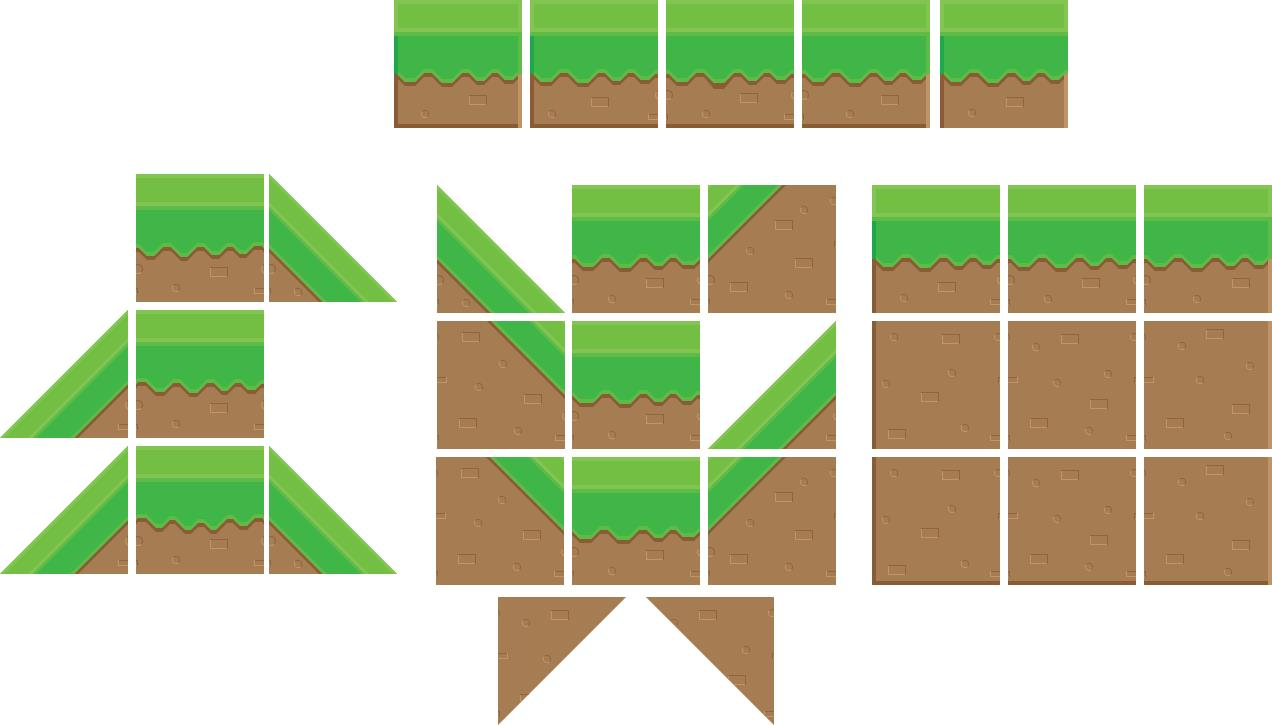
\includegraphics[scale=0.25]{kepek/tileMap/TileSet.png}
			\caption{Platform játékhoz alkalmas tileset}
			\label{fig:tileMap:tileSet}
		\end{figure}
	
		A Tile-Map alapú megjelenítésre a legalkalmasabb játéktípusok között vannak a felülnézetes, a puzzle, vagy például a platformer játékok. (A fentebbi tileset és egyéb elemek használatával példa a megjelenítési technikára: \myref{fig:tileMap:tileMapPreview} ábra)
		\begin{figure}[h!]
			\centering
			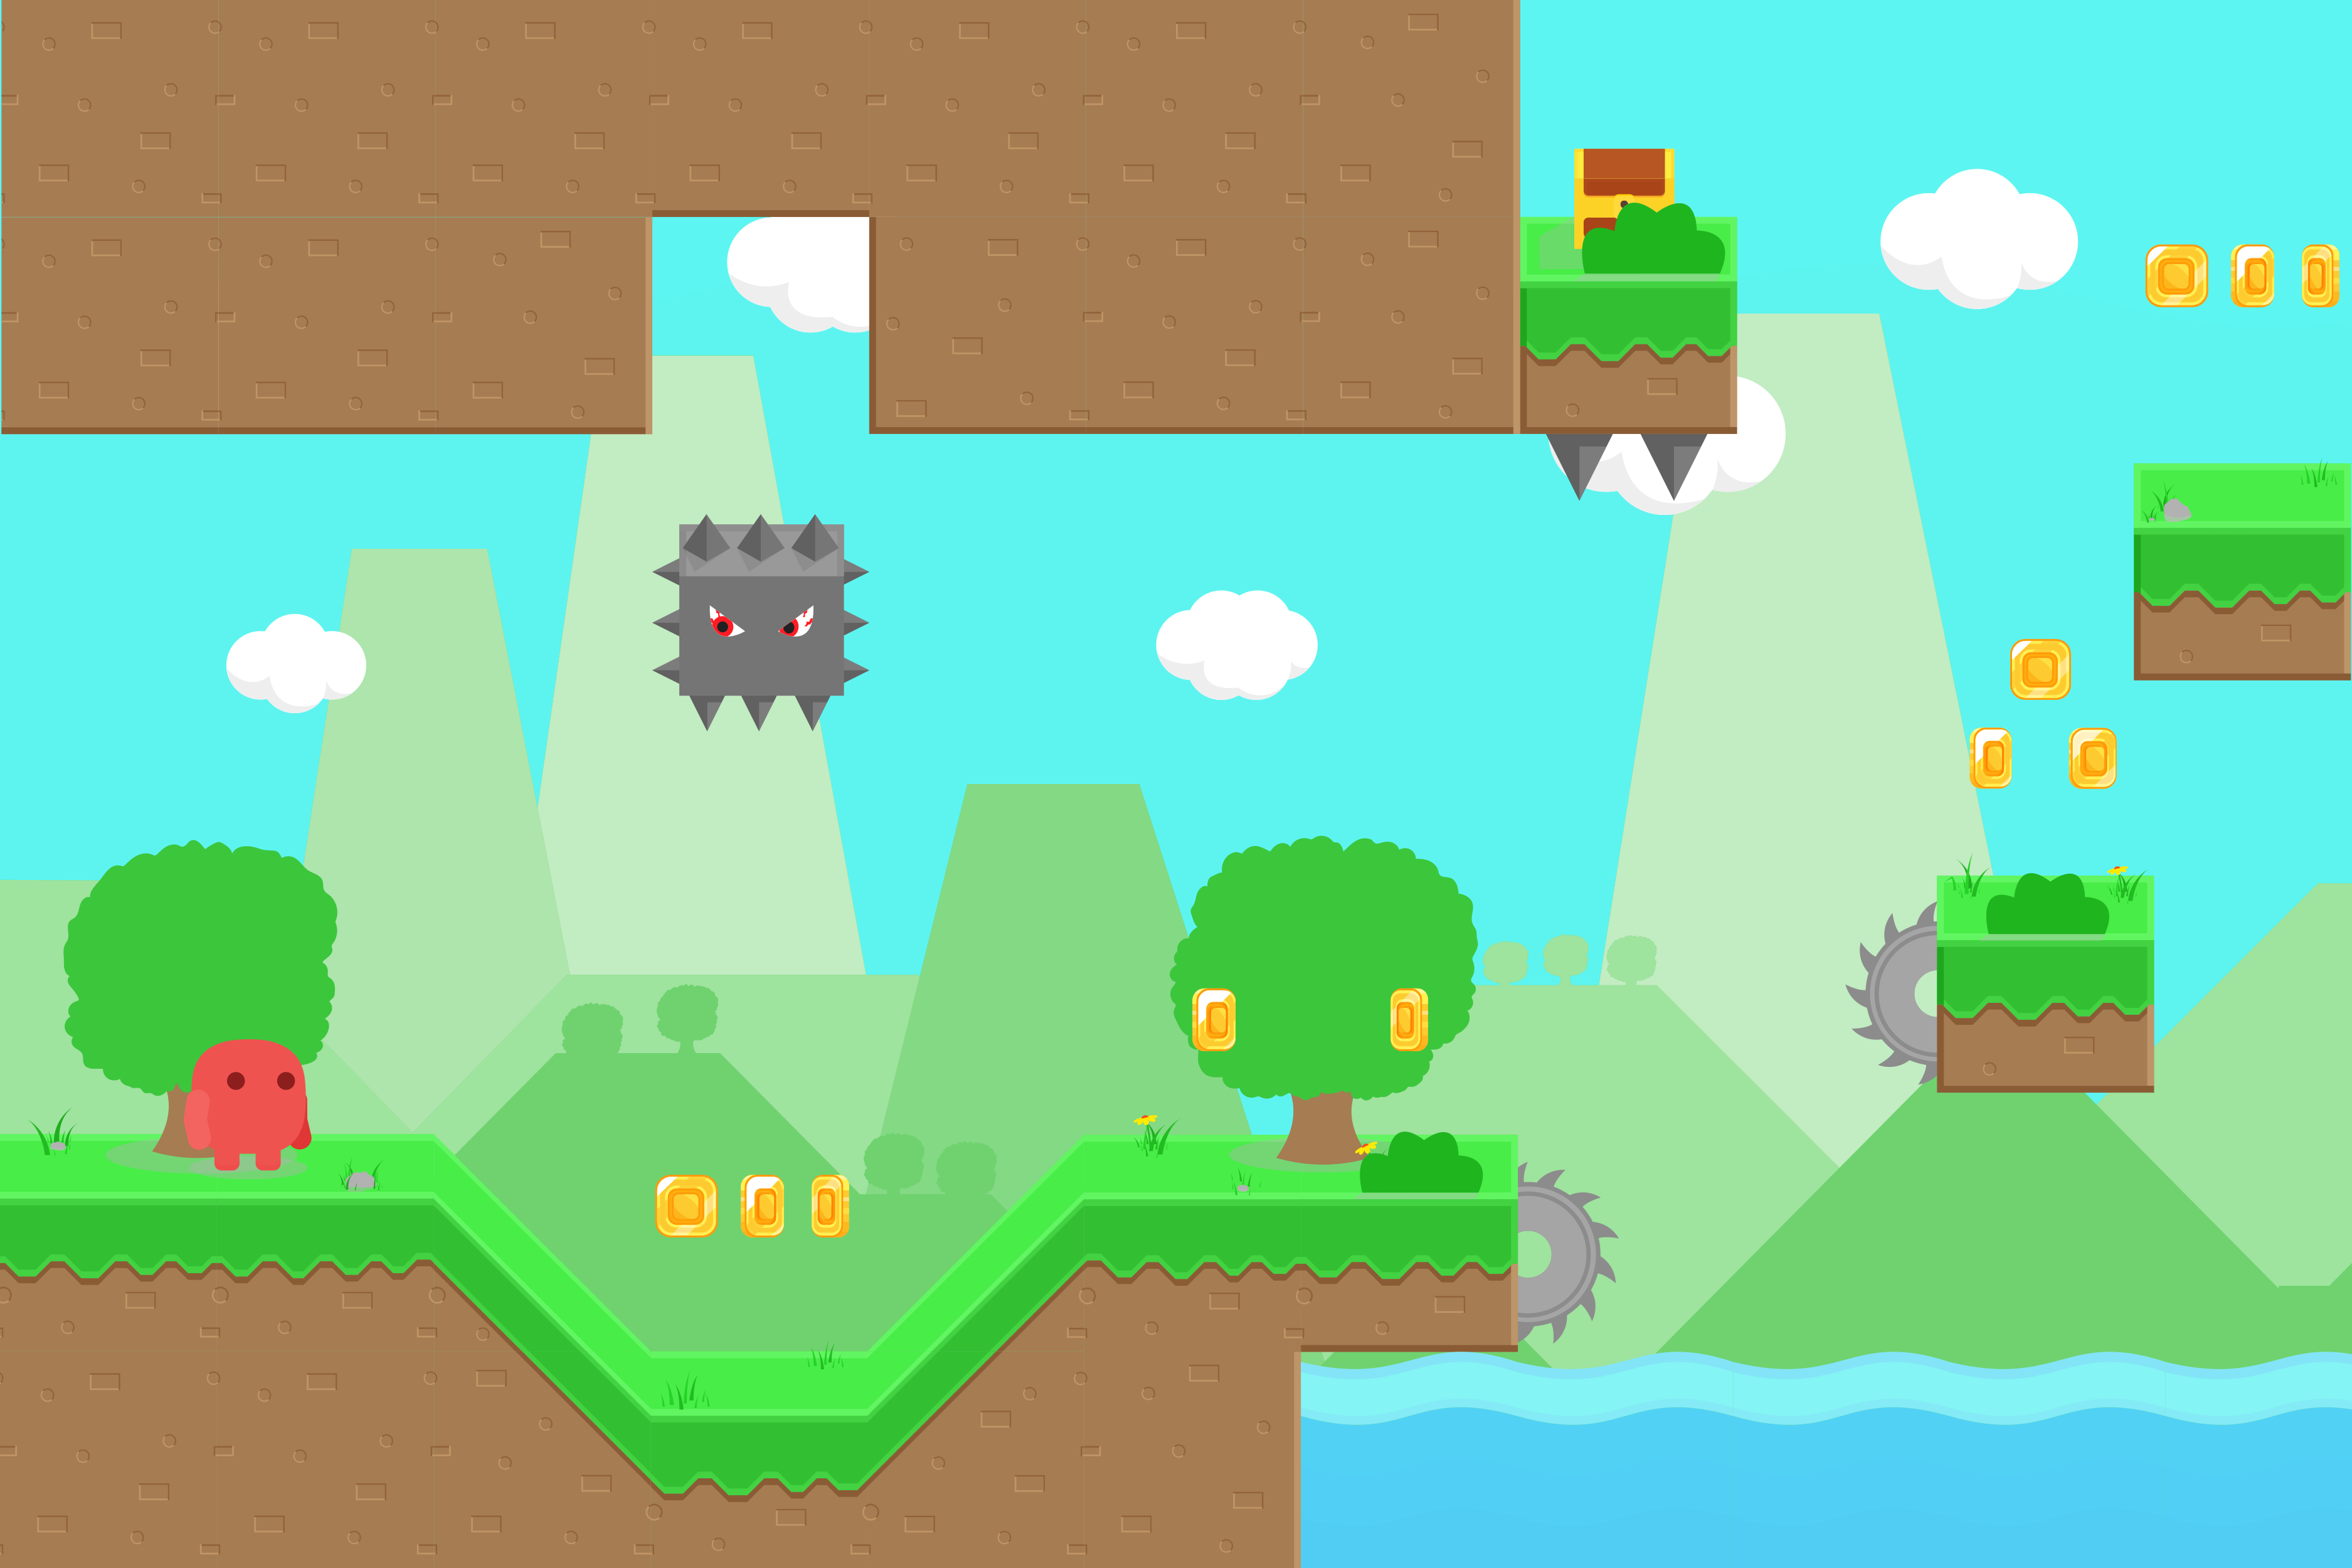
\includegraphics[scale=0.35]{kepek/tileMap/TileMapPreview.png}
			\caption{Példa tilesettel létrehozott platform játékra}
			\label{fig:tileMap:tileMapPreview}
		\end{figure}
		% TODO irodalom ->
		% https://bayat.itch.io/platform-game-assets
	\end{MySection}

	\begin{MySection}{Webes játékfejlesztés keretrendszerek nélkül}
		% TODO 	- "pure js"-ben
		% TODO 	- webgl
	\end{MySection}

	\begin{MySection}{Webes játékfejlesztés keretrendszerekkel}
		% TODO 	- keretrendszerek miért jók
		% TODO 	(- összehasonlítás menete(?))
		% TODO 	- felsorolni (tovább bontani al-al-fejezetekre ha megoldható)
		% TODO 	- megemlíteni melyik miért jó, miben más, használatuk, esetleg kipróbálás, személyes tapasztalatok
		% TODO 	- összehasonlítás eredménye / összegzése az előzőnek
		% TODO 	- dönteni melyiket használom -> Phaser 3 -> ezzel kapcsolatos tapasztalatokat(általánosan h erre a célra mennyire felel meg, ajánlanám-e ezt ilyen jellegű program készítésére)
		
		Keretrendszerek használatával hatékonyabban, gyorsabban lehetünk képesek egy játék elkészítésére, kimondottan kezdőként könnyebben szerezhetünk tapasztalatot játékmotor használatával, mint anélkül.
		
		Amennyiben valaki játékfejlesztés előtt áll, és úgy dönt, hogy keretrendszert fog alkalmazni az alkalmazás elkészítéséhez, még rengeteg átgondolnivalója van, például abban a tekintetben, hogy melyik motort fogja használni. Fontos, hogy megtaláljuk a célunkhoz legmegfelelőbb keretrendszert. A választást rengeteg dolog befolyásolhatja, például az elkészíteni kívánt játék grafikája, a preferált programnyelv, vagy hogy mennyire nehéz egy-egy keretrendszer használatának elsajátítása, satöbbi. A lehetőségek felméréséhez segítség lehet például egy-egy tömör összefoglalást átolvasni az egyes motorokról, vagy ha az időnk engedi kipróbálni, tapasztalatokat gyűjteni róluk, majd azután összevetni őket.
		
		\begin{MySubSection}{Játékmotorok összehasonlítása}
			A most következő részben különféle játékfejlesztéshez használható HTML5 alapú keretrendszereket fogok összehasonlítani röviden, hogy egy kis áttekintést kapjunk néhány lehetséges motorral kapcsolatosan. Számomra most egyrészt az a fontos, hogy ingyenesen használható legyen a motor, másrészt, mivel 2D-s játékot szeretnék készíteni, az is lényeges, hogy egy erre jobban alkalmas keretrendszert használjak, ne pedig három dimenziós játékok fejlesztésére készített játékmotort. 
			Ezek a feltételek már önmagukban leszűkítették a szóba jöhető keretrendszerek körét, de az egyes motorok dokumentációit és a felhasználói véleményeket is figyelembe fogom venni a választás során. Végül négy játékmotor volt, amik szimpatikusabbak voltak, így jobban utánuk néztem, ezekről fogok pár szót írni, majd pedig eldönteni, hogy melyiket fogom használni a játék elkészítéséhez.
			
			A négy összehasonlítandó keretrendszer:
			
			\begin{itemize}
				\item \textit{ImpactJS}, \url{https://impactjs.com/}
				\item \textit{Phaser}, \url{https://phaser.io/}
				\item \textit{Modd.io}, \url{https://www.modd.io/}
				\item \textit{GDevelop}, \url{https://gdevelop-app.com/}
			\end{itemize}
		\end{MySubSection}
	
		\begin{MySubSection}{ImpactJS Engine}
		\end{MySubSection}
	
		\begin{MySubSection}{Phaser}
		\end{MySubSection}
		
		\begin{MySubSection}{Modd.io}
		\end{MySubSection}
		
		\begin{MySubSection}{GDevelop}
		\end{MySubSection}
		
	\end{MySection}
	
\end{MyChapter}